\chapter[Sistema Adaptativo de Vídeos Interativos]{Sistema Adaptativo de Vídeos Interativos}

Tendo como base as teorias apresentadas, foi desenvolvido um sistema que utiliza o modelo arquitetural MVC e que contempla duas funcionalidades principais: um módulo para autoria de cursos compostos por vídeos interativos e um módulo para visualização adaptativa destes cursos, que contemple adaptações de conteúdo e navegação. Este capítulo apresenta os resultados obtidos no desenvolvimento, englobando o módulo de autoria de cursos, o módulo de visualização adaptativa e o mecanismo de quantização por meio da QRN.

\section{Módulo de Autoria de Cursos}

O módulo de autoria de cursos tem o propósito de permitir que educadores construam materiais de estudo para enriquecer a base de dados do sistema proposto. Este módulo pode ser mais facilmente compreendido se dividido em dois níveis: o nível conceitual e o nível de construção do hypervideo.

No nível conceitual, o professor poderá criar um novo curso, seus hipervideos e as ligações entre eles, construindo assim, a rede na qual o estudante navegará. Este nível representa o mapa conceitual que aparecerá para o estudante quando pesquisar um curso no sistema, sendo de extrema importância, pois, o aprendizado é mais efetivo se o estudante tiver conhecimento do todo antes das partes.

\begin{figure}[h!]
  	\centering
  	\begin{subfigure}{.5\textwidth}
  		\centering
  		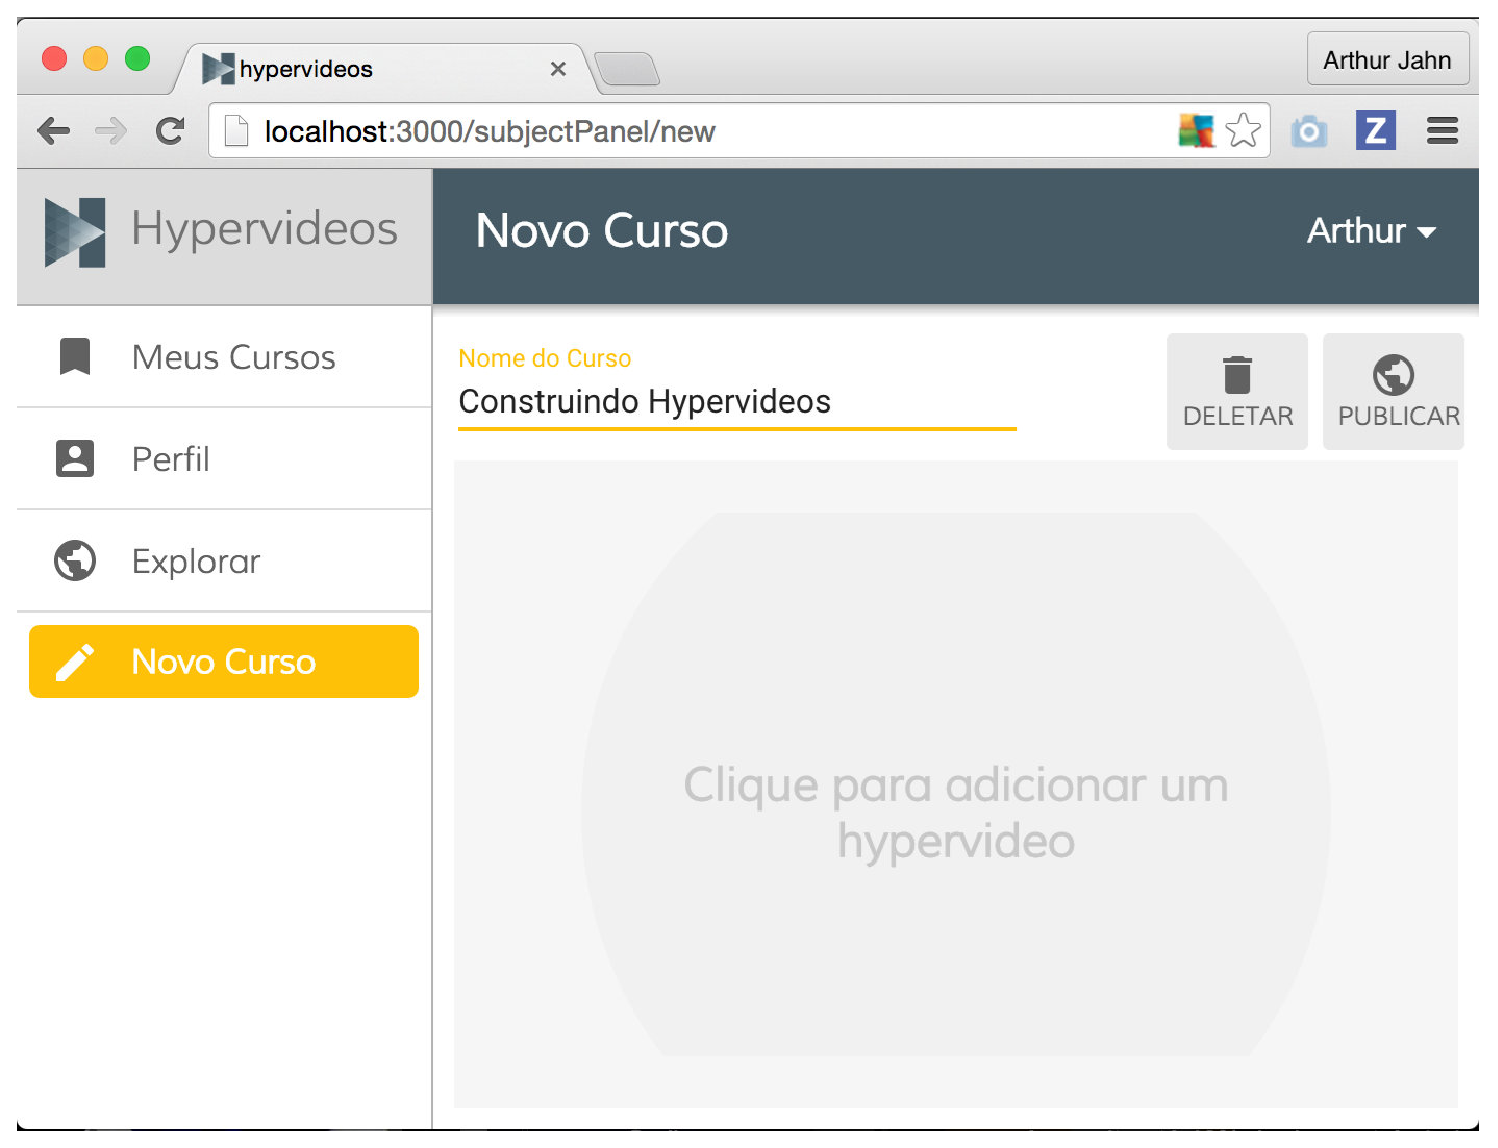
\includegraphics[width=.9\linewidth]{figuras/autoria_conceitual_a.eps}
  		\caption{Adição de título ao curso.}
  		\label{fig:autoria_conceitual_a}
	\end{subfigure}%
	\begin{subfigure}{.5\textwidth}
  		\centering
  		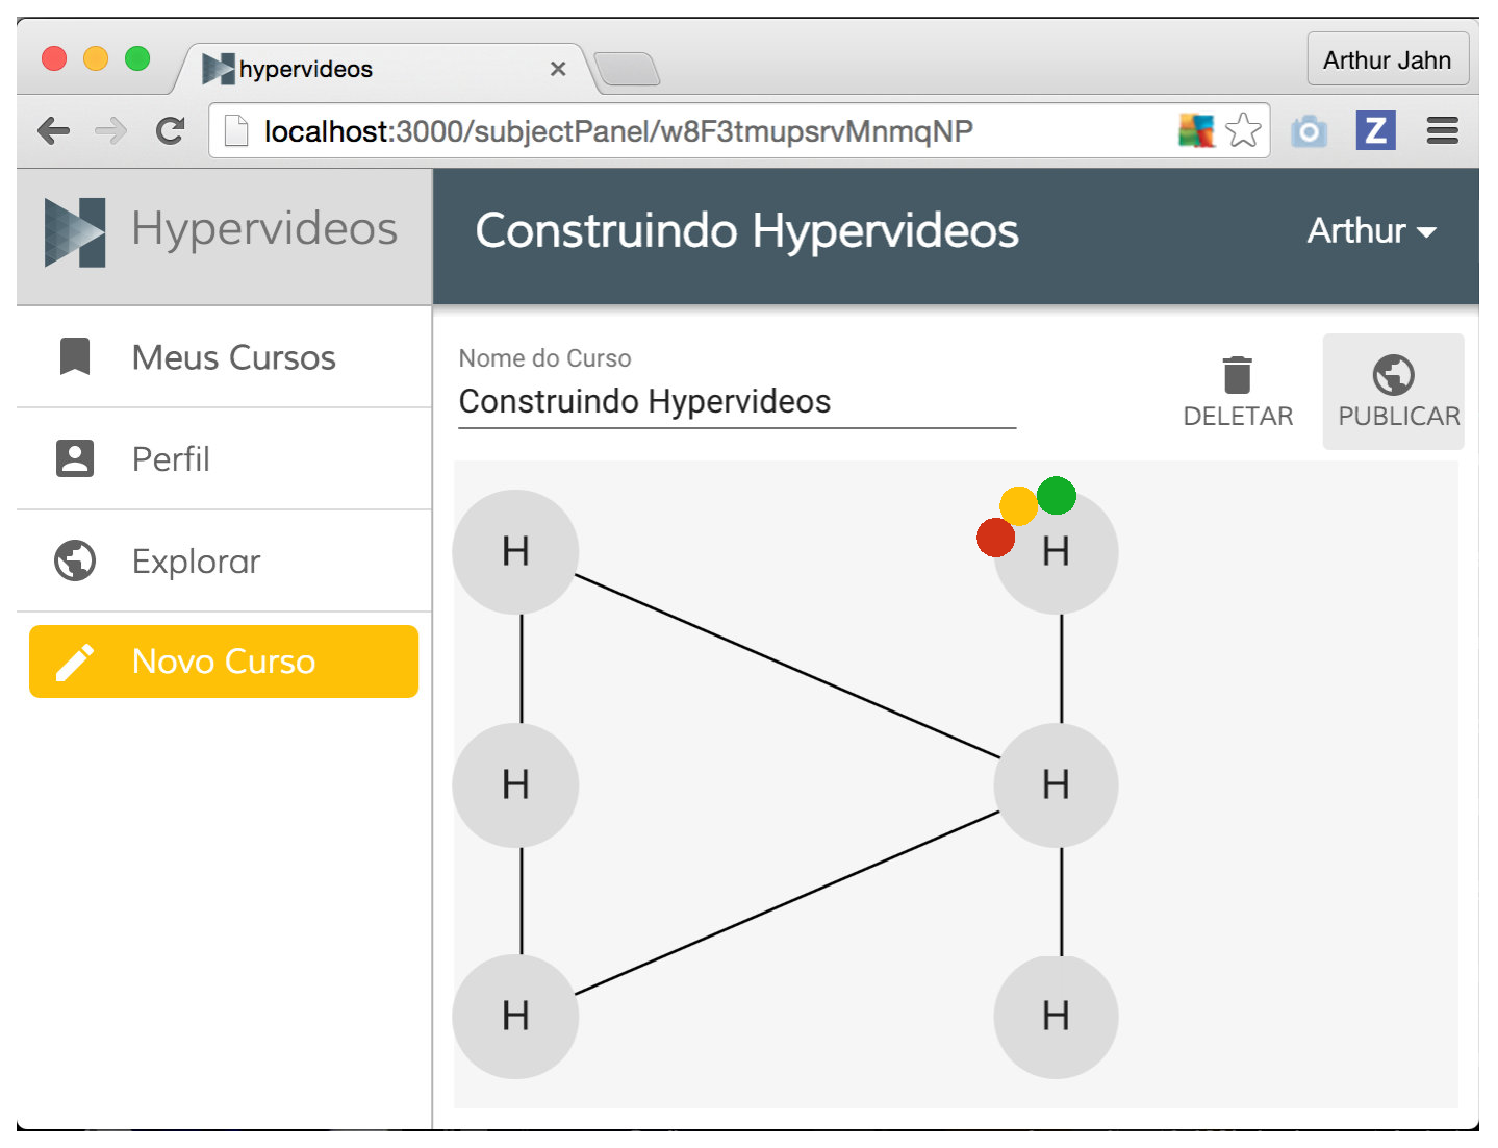
\includegraphics[width=.9\linewidth]{figuras/autoria_conceitual_b.eps}
  		\caption{construção do mapa conceitual.}
  		\label{fig:autoria_conceitual_b}
	\end{subfigure}%
	
	\begin{subfigure}{.5\textwidth}
  		\centering
  		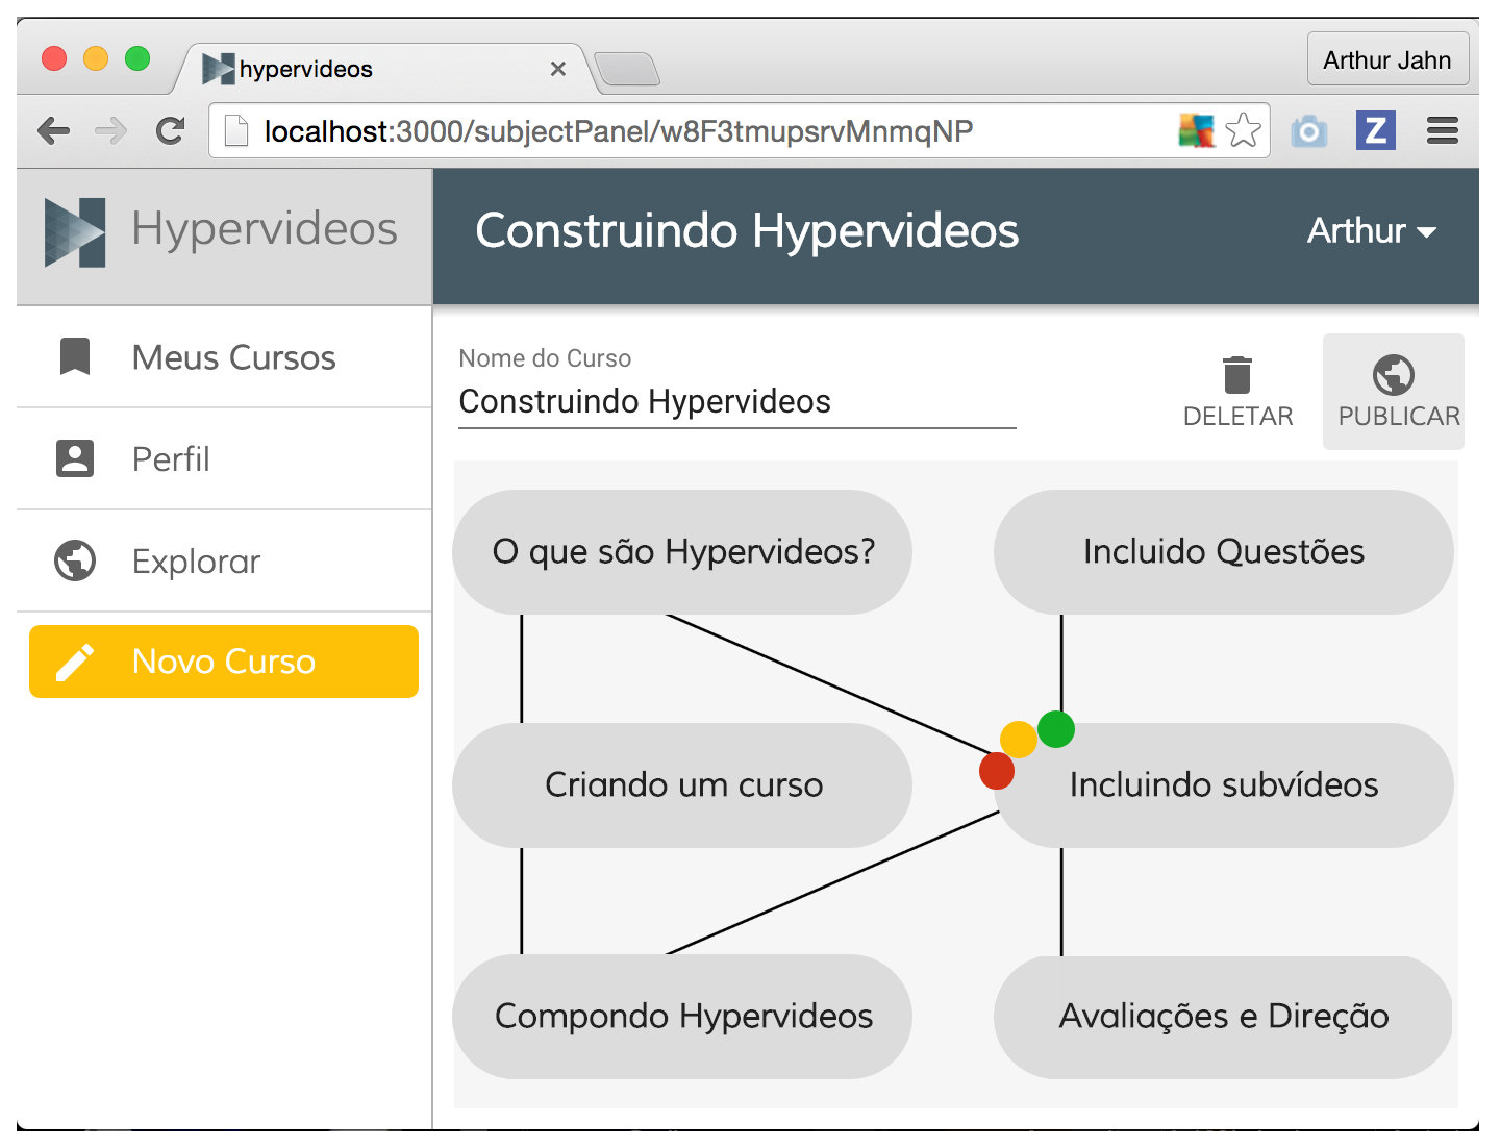
\includegraphics[width=.9\linewidth]{figuras/autoria_conceitual_c.eps}
  		\caption{visualização dos conceitos.}
  		\label{fig:autoria_conceitual_c}
	\end{subfigure}%
	\begin{subfigure}{.5\textwidth}
  		\centering
  		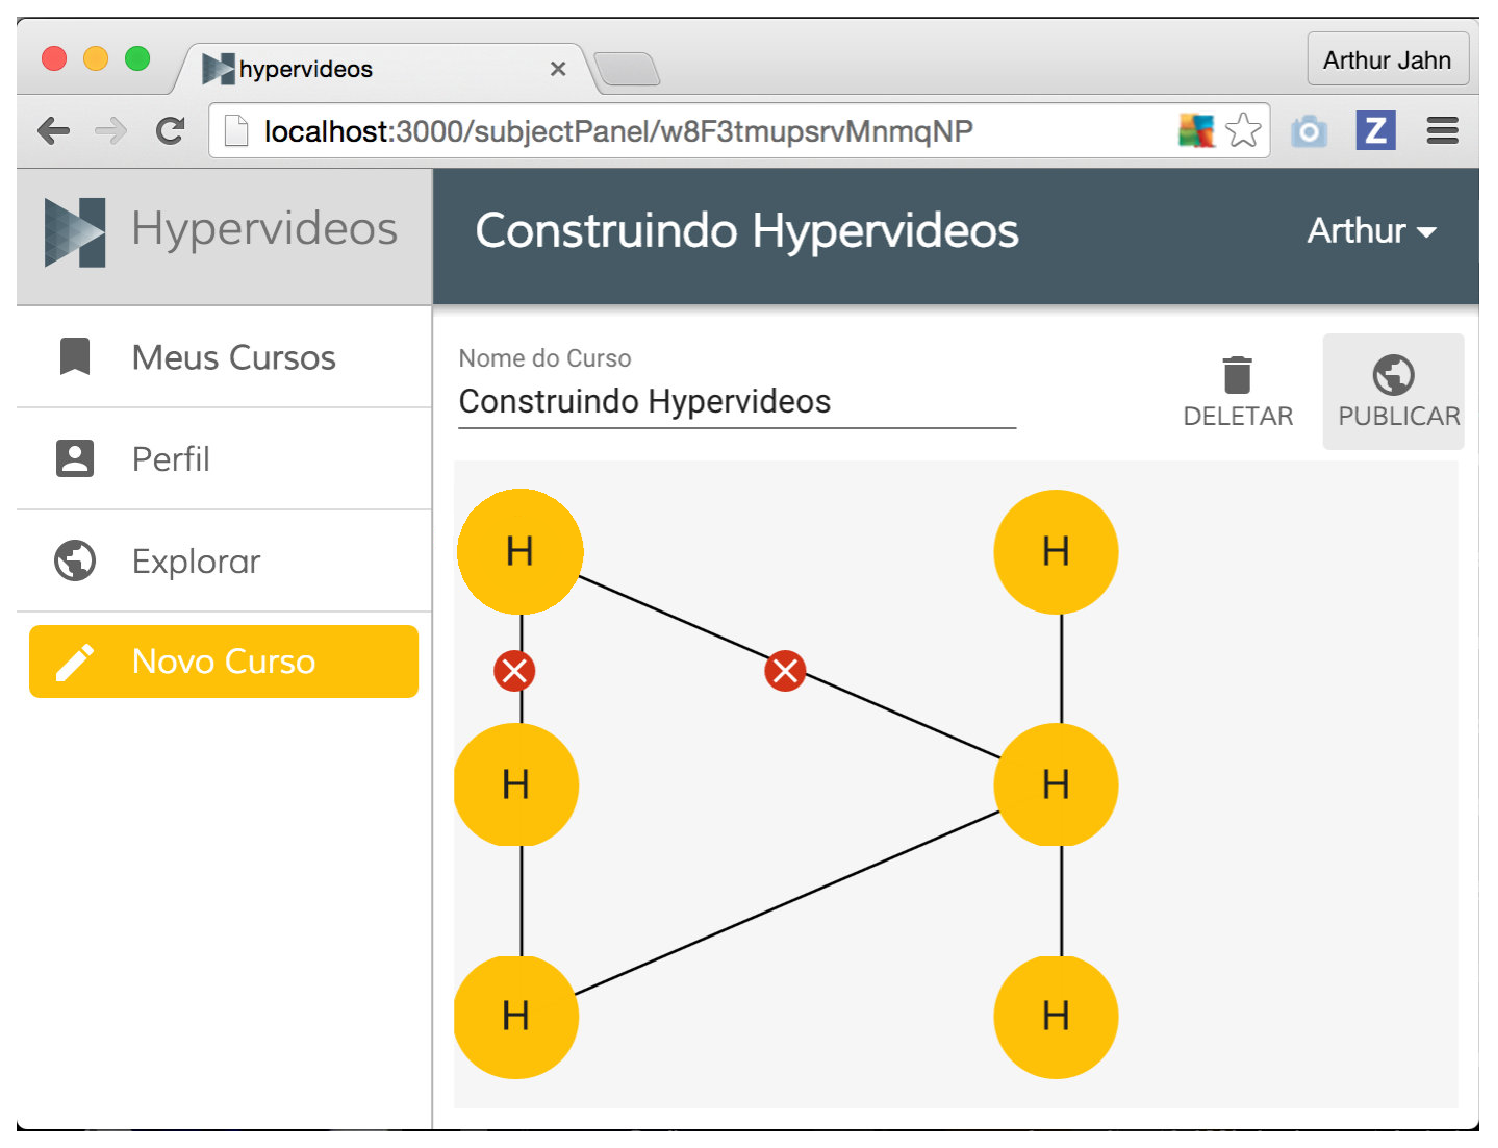
\includegraphics[width=.9\linewidth]{figuras/autoria_conceitual_d.eps}
  		\caption{modo de edição de ligações.}
  		\label{fig:autoria_conceitual_d}
	\end{subfigure}%
  	\caption{Funções do módulo de autoria no nível conceitual.}
  	\label{fig:autoria_conceitual}
\end{figure}

A figura \ref{fig:autoria_conceitual_a} mostra o componente de criação de um curso, no qual existe um campo para a definição do título e uma área central que permite a composição do mapa conceitual, por meio da adição, remoção, interligação ou edição de cada hypervideo adicionado durante a construção do curso.

Novos hypervideos podem ser adicionados clicando na área de composição do curso. A figura \ref{fig:autoria_conceitual_b} ilustra um mapa construído, no qual podem ser visualizados os ícones que representam hypervideos. Clicando em um hypervideo criado, é possível ver o conceito definido para ele, como ilustra a figura \ref{fig:autoria_conceitual_c}, com todos os conceitos do mapa visíveis. A figura \ref{fig:autoria_conceitual_d}  mostra o mapa conceitual em modo de ligação, para permitir a criação e deleção de \textit{links} entre hypervideos.

É possível visualizar nas figuras \ref{fig:autoria_conceitual_b} e \ref{fig:autoria_conceitual_c}, três botões coloridos sobre o ícone de um hypervideo. Esses botões aparecem quando o cursor passa sobre o ícone e permitem que o usuário execute as seguintes ações: remover o hypervervídeo (botão vermelho), criar conexões para o hypervideo (botão amarelo) ou construir o conteúdo do hypervídeo (botão verde), esta última sendo discutida a seguir. 

No nível de construção do conteúdo de um hypervideo é possível adicionar subvídeos e questões para criar a navegação no hypervideo. 

\begin{figure}[h!]
  	\centering
  	\begin{subfigure}{.5\textwidth}
  		\centering
  		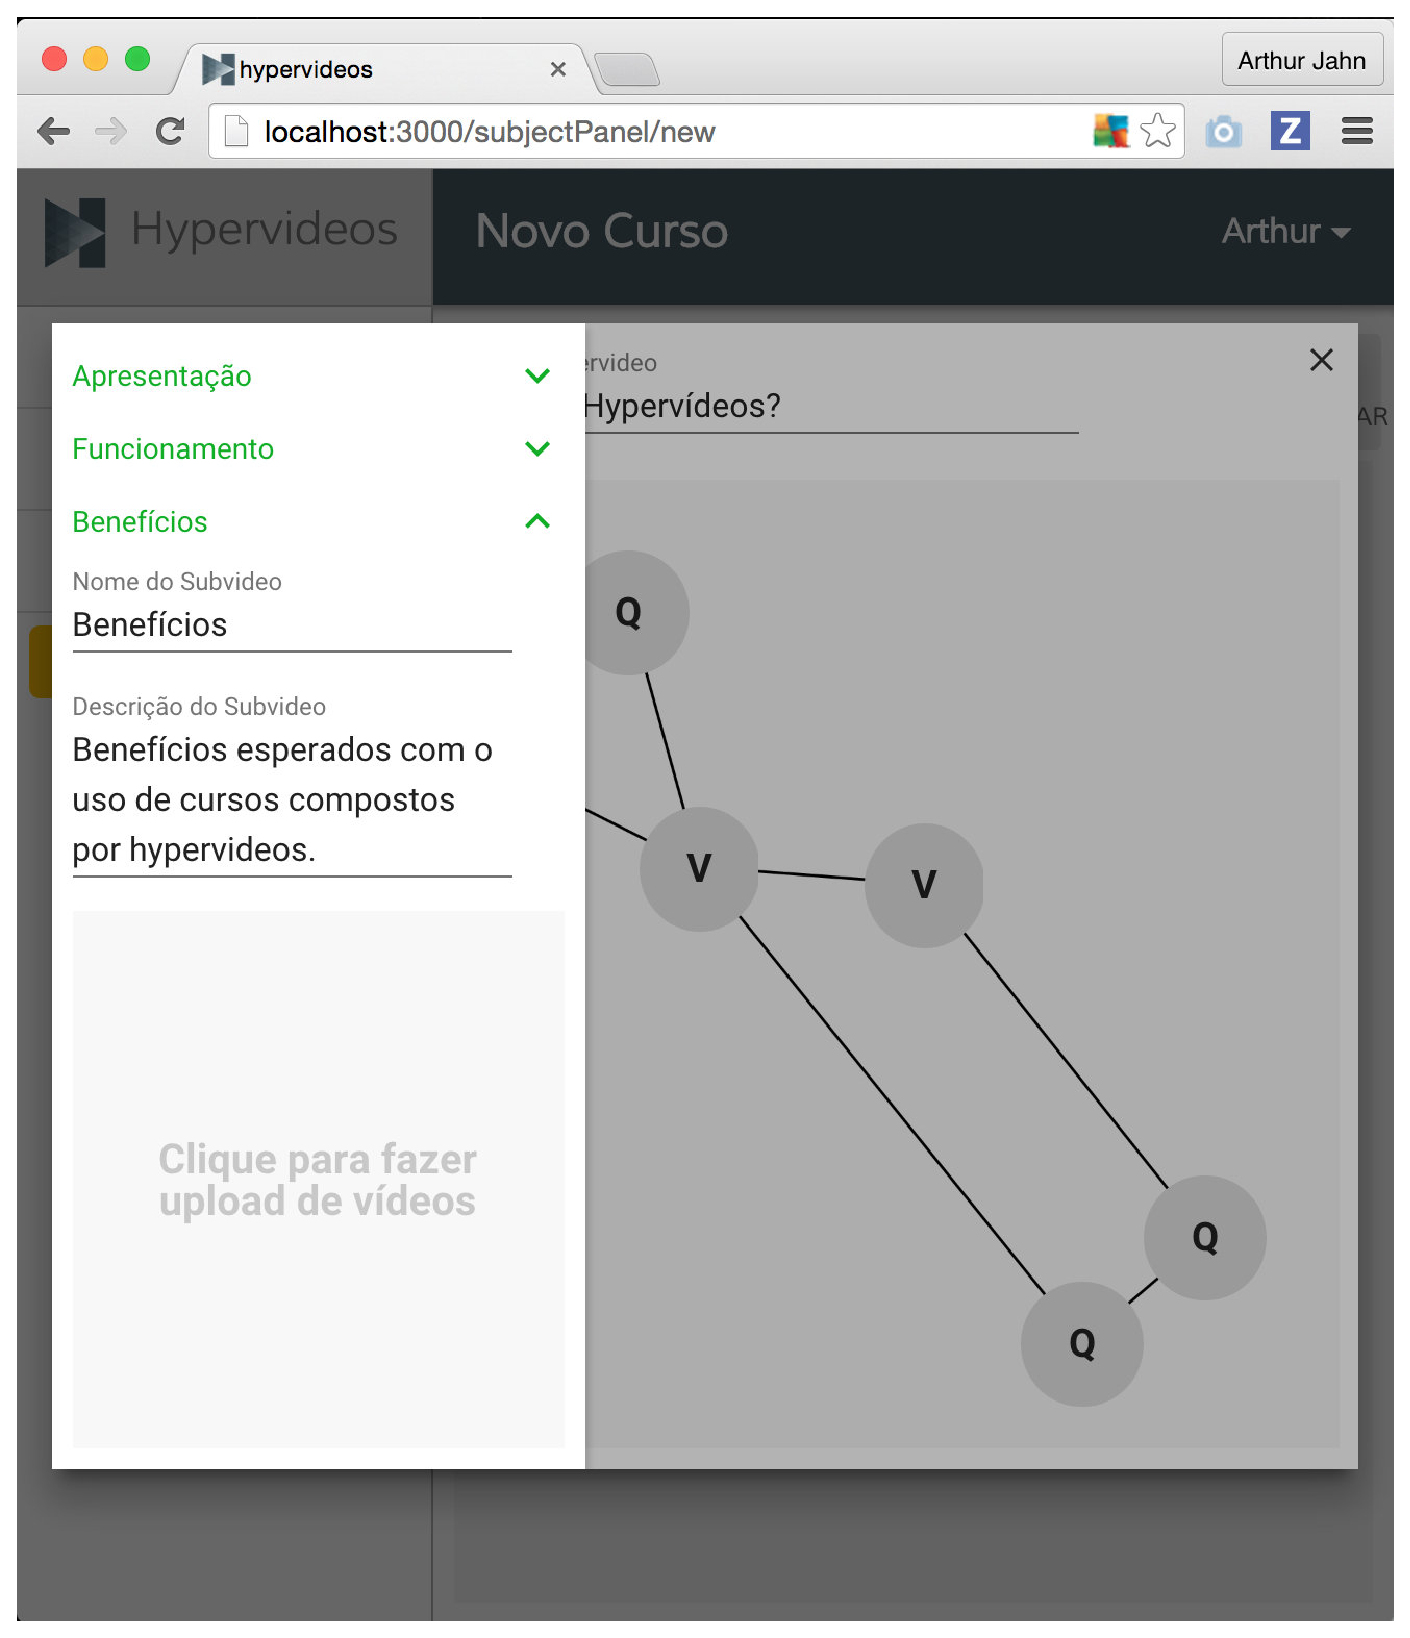
\includegraphics[width=.95\linewidth]{figuras/autoria_construcao_a.eps}
  		\caption{Subvídeos carregados.}
  		\label{fig:autoria_construcao_a}
	\end{subfigure}%
	\begin{subfigure}{.5\textwidth}
  		\centering
  		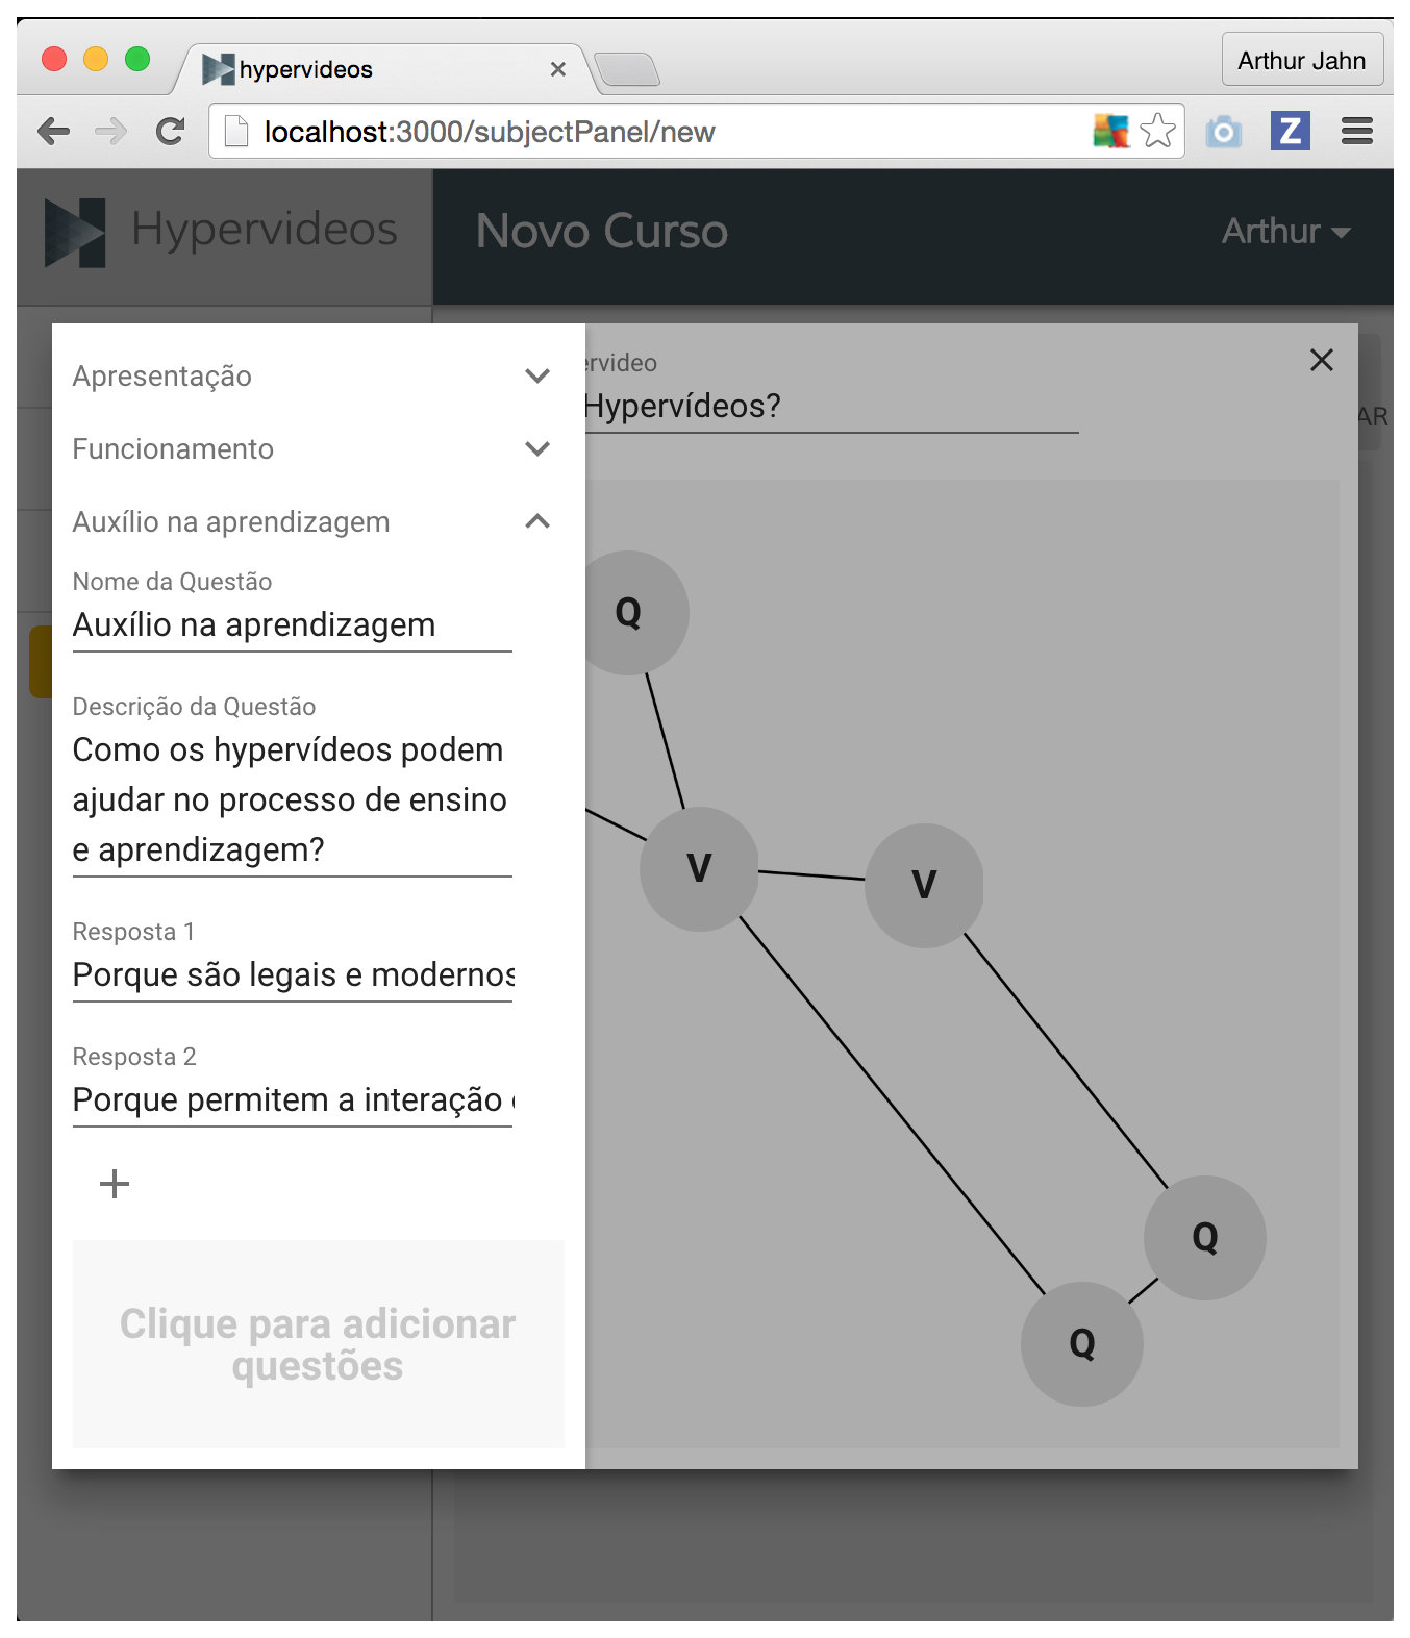
\includegraphics[width=.95\linewidth]{figuras/autoria_construcao_b.eps}
  		\caption{Questões criadas.}
  		\label{fig:autoria_construcao_b}
	\end{subfigure}%
  	\caption{Funções do módulo de autoria no nível de construção do hypervideo.}
  	\label{fig:autoria_construcao}
\end{figure}

Subvídeos são criados por meio do carregamento de arquivos de vídeo na aba de vídeos e criam automaticamente questões vinculadas. O sistema permite também que mais questões sejam criadas dentro da aba de questões. 

Subvídeos e questões possuem um nível de visibilidade para restringir que materiais muito complexos ou muito simples apareçam para o usuário que assiste ao curso. A figura \ref{fig:autoria_construcao} apresenta a página de composição de um hypervídeo com três subvídeos (fig. \ref{fig:autoria_construcao_a}) e três questões (fig. \ref{fig:autoria_construcao_b}), ao fundo da figura é possível ver o grafo de conexões do hypervideo.

Após a construção de todos os hypervídeos, o autor poderá publicar o curso na rede e a partir desse momento, outros usuários poderão assistir ao material educativo. Essa parte da interação é apresentada no tópico seguinte, a respeito do módulo de visualização adaptativa.

\section{Módulo de Visualização Adaptativa}

O módulo de visualização adaptativa permite que o usuário assista um curso disponibilizado na rede de acordo com seu nível no sistema. As operações executadas pelo usuário neste módulo começam no momento da busca por um curso. Na página "Explorar", é possível assistir a um curso ou adicioná-lo à biblioteca para assistir depois, como mostra a figura \ref{fig:explorar}.

\begin{figure}[h!]
  	\centering
  	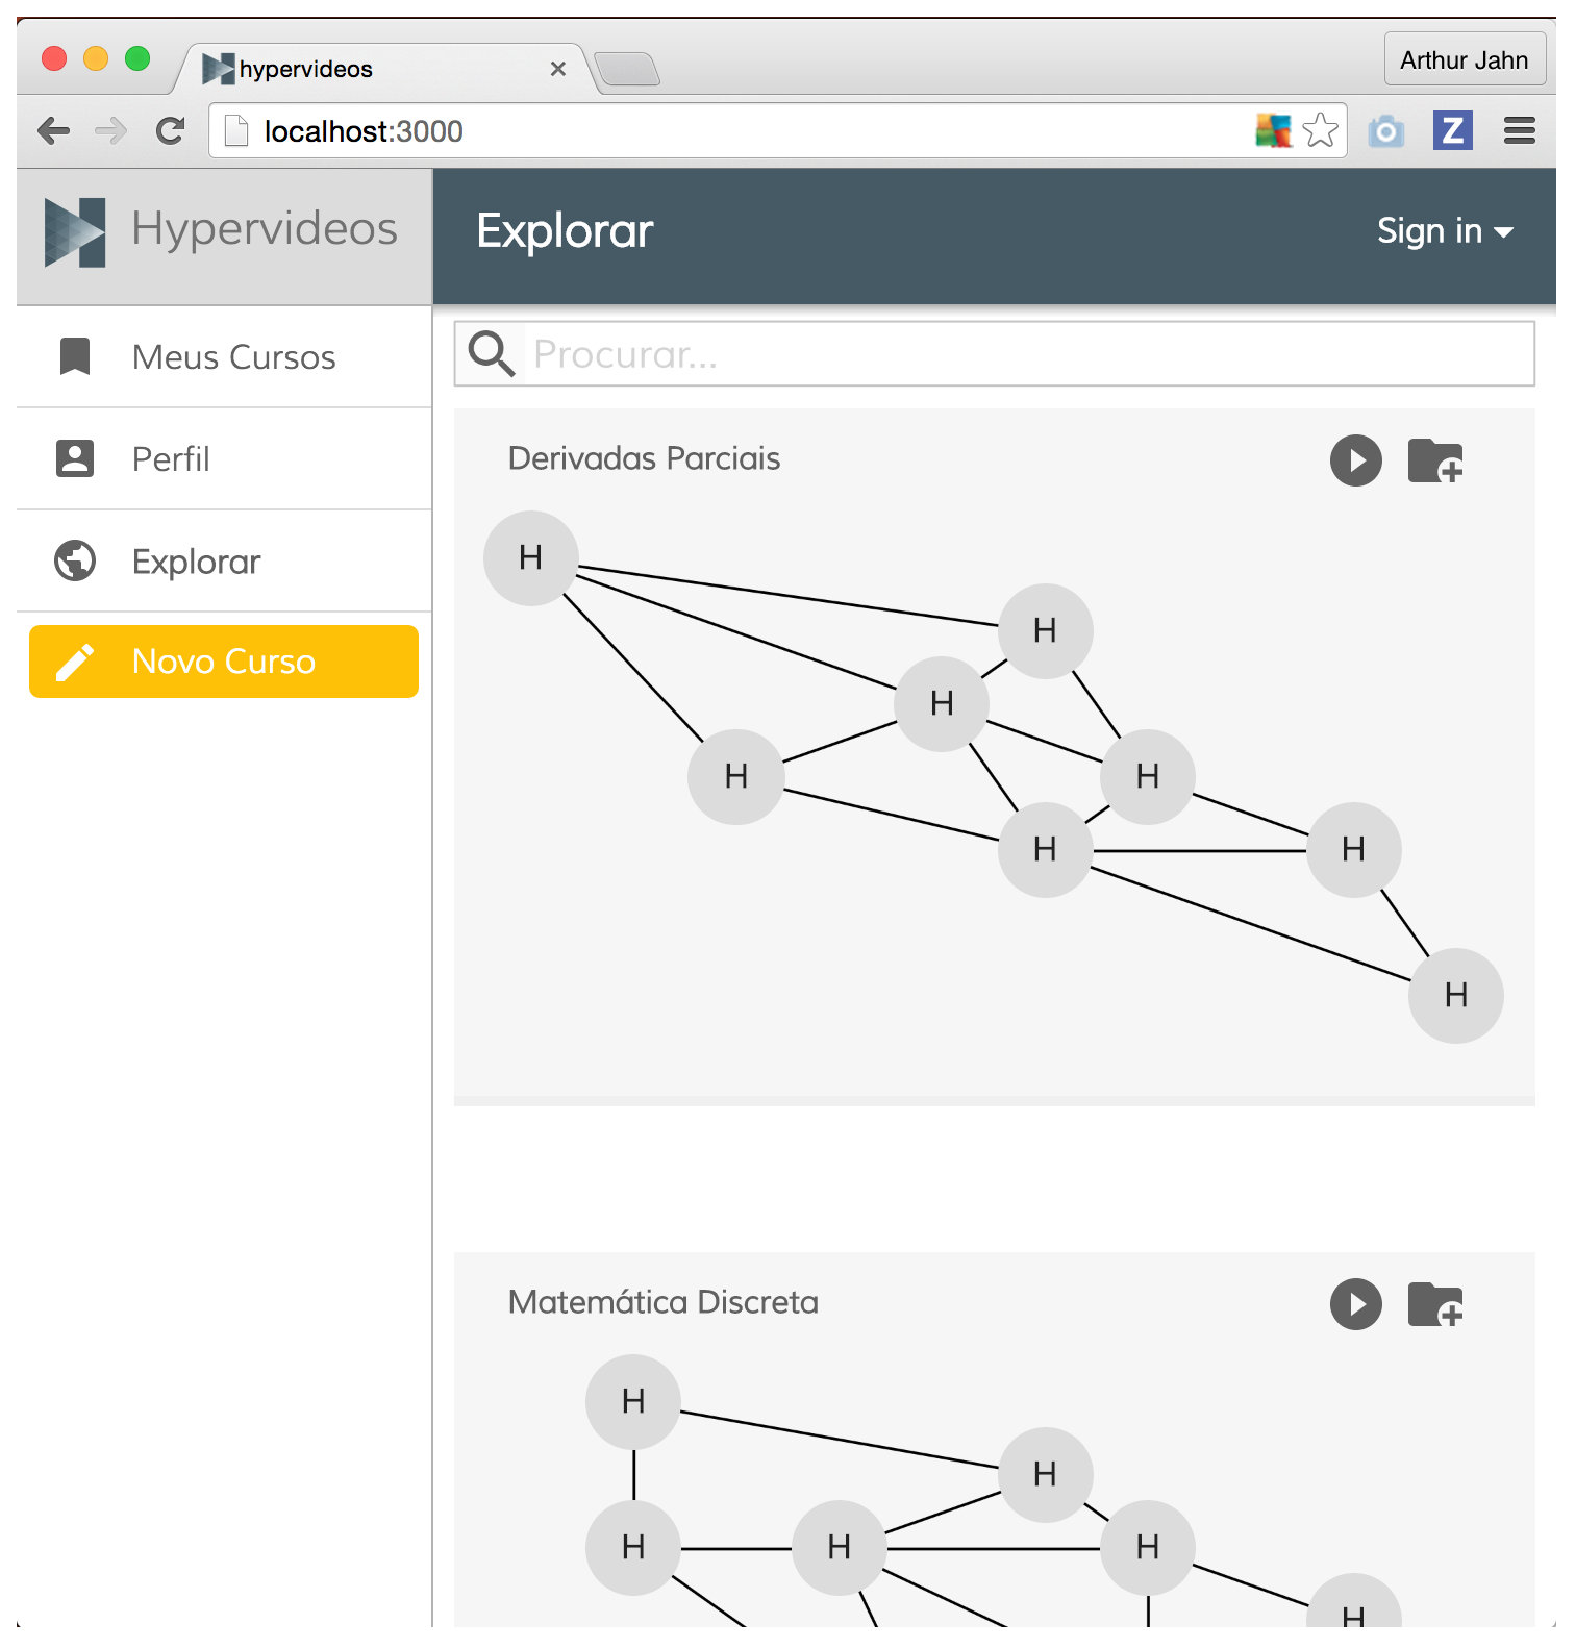
\includegraphics[width=.6\linewidth]{figuras/explorar.eps}
  	\caption{Página de busca por cursos.}
  	\label{fig:explorar}
\end{figure}

Quando o usuário opta por assistir um curso, ele é direcionado para a página de apresentação adaptativa, como mostra a figura \ref{fig:apresentar}. Nesse ambiente, o usuário é capaz de responder às questões propostas pelo professor, selecionar subvídeos de sua preferência e visualizar seu progresso no fluxo do curso.

\begin{figure}[h!]
  	\centering
  	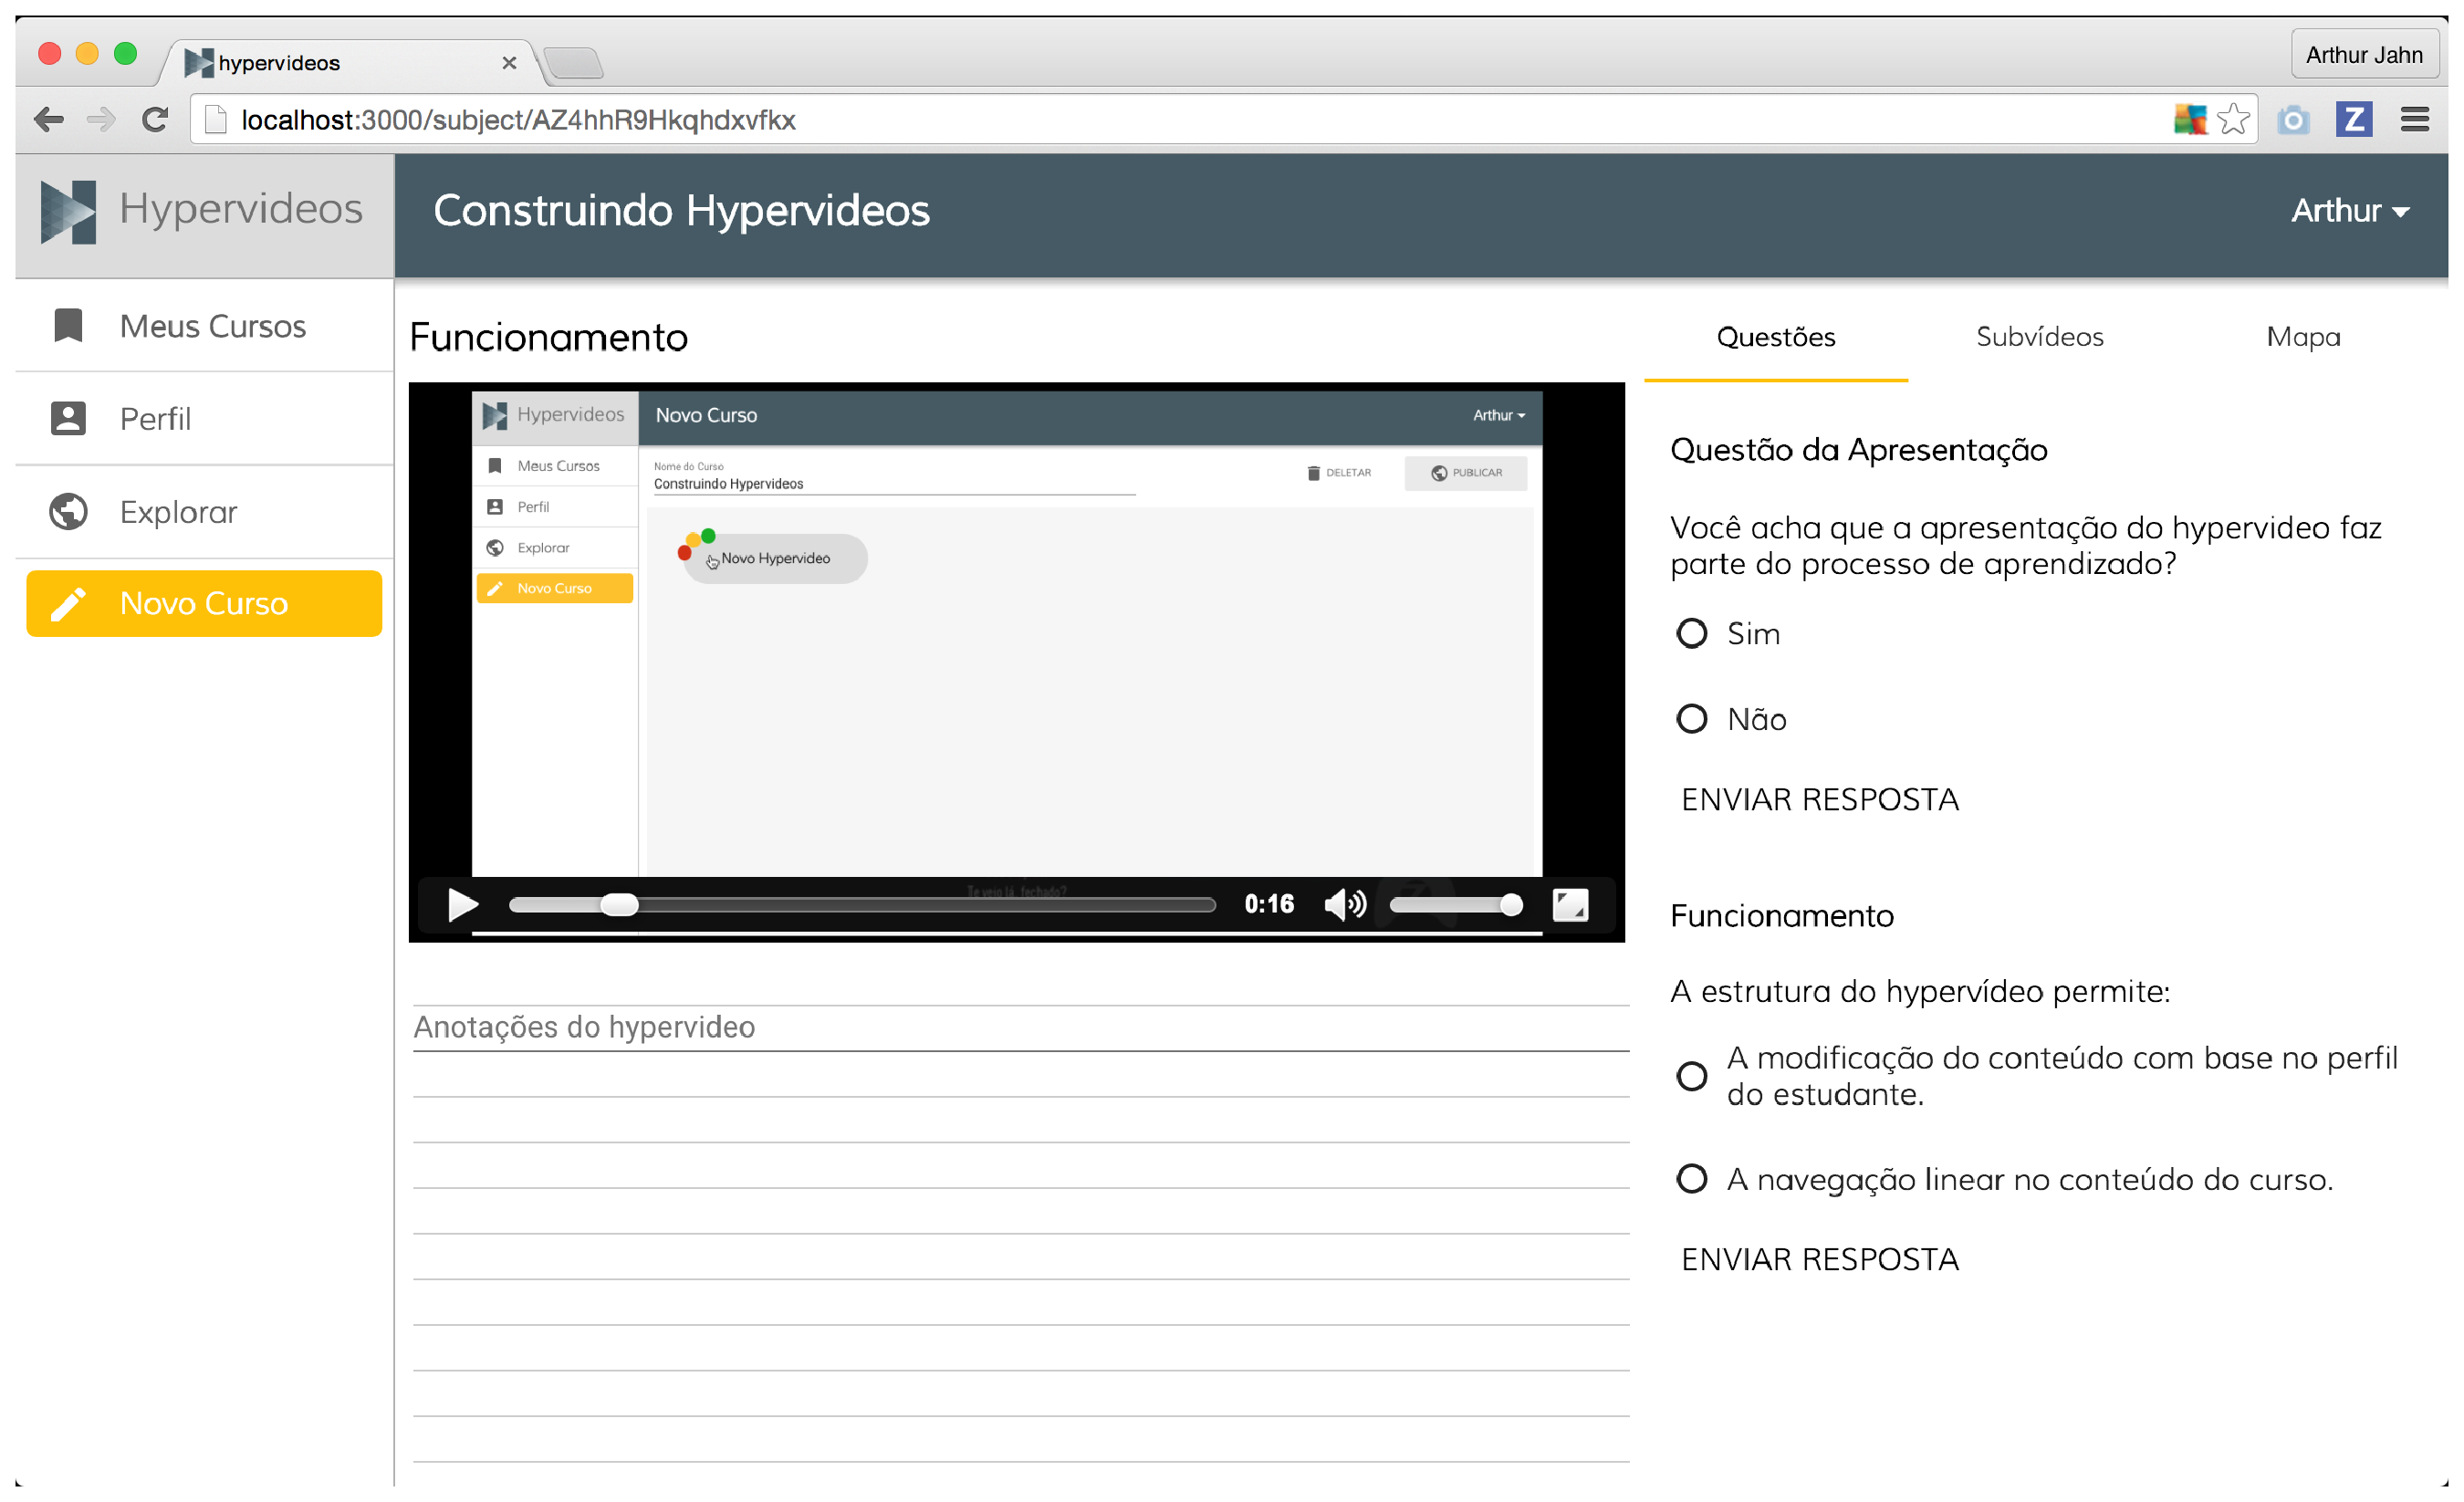
\includegraphics[width=.9\linewidth]{figuras/apresentar.eps}
  	\caption{Módulo de visualização adaptativa.}
  	\label{fig:apresentar}
\end{figure}

O módulo de visualização possui um componente para que o usuário possa fazer anotações sobre o hypervideo, que servem de suporte para o aprendizado do conteúdo apresentado. É importante ressaltar que a adaptação do conteúdo foi alcançada por meio do filtro dos subvídeos e questões segundo o perfil do usuário, que aparecem nas abas ao lado do reprodutor de vídeo, juntamente com o mapa do curso.

\section{Mecanismo de Quantização por meio da QRN}

O mecanismo de quantização permite que a navegação entre hypervideos de um curso seja adaptativa de acordo com os escores obtidos pelo estudante, a confiabilidade da avaliação, o decaimento temporal e as ligações que o hypervideo possui. Esse cálculo é feito unicamente no servidor, que envia a resposta das operações para o cliente, permitindo assim, que outros hypervideos sejam indicados pelo sistema. 

\begin{figure}[h!]
  	\centering
  	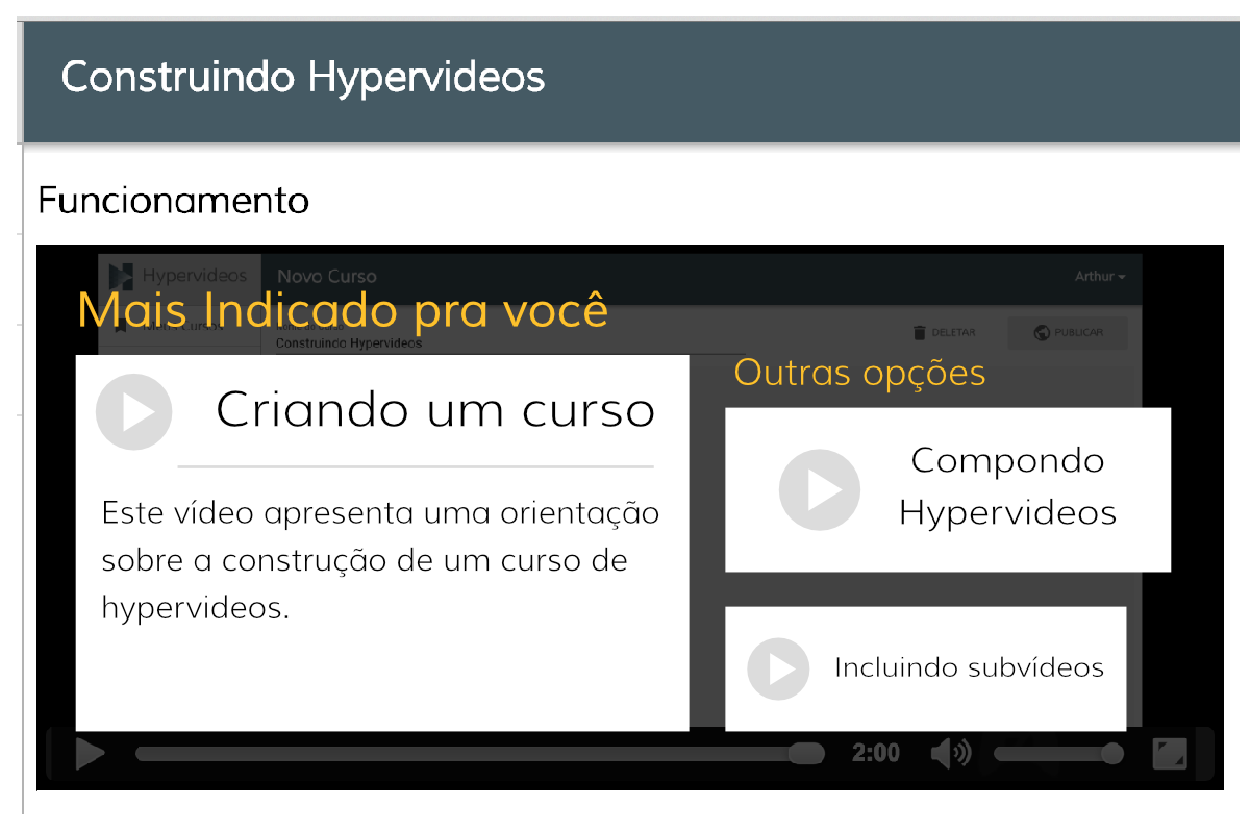
\includegraphics[width=.5\linewidth]{figuras/quantizacao.eps}
  	\caption{Componente de apresentação dos hypervideos indicados.}
  	\label{fig:quantizacao}
\end{figure}

O \textit{Meteor} permite essas operações por meio de métodos (i.e. \textit{Meteor Methods}) executados unicamente no servidor e simulados no cliente, que é atualizado quando a operação no servidor é concluída e devolvida. Na arquitetura do sistema, esses métodos são chamados pelo modelo, o que faz sentido, já que são operações da lógica do domínio da aplicação e compõem a parte do modelo que está definida no servidor. O componente de apresentação dos hypervideos sugeridos pelo sistema aparece como mostrado na figura \ref{fig:quantizacao}.

Apesar do componente de apresentação dos hypervideos indicados estar construído, até o momento da escrita deste trabalho não foi possível validar a implementação da QRN com um curso real no sistema, apenas por meio de inspeção e validação das equações utilizadas. Isso devido aos coeficientes para indicar a direção da evolução no curso e também, ao coeficiente relacionado aos blocos coesos, representados por meio das ligações entre hypervideos, que necessita ser calibrado para não impossibilitar que outros nodos da rede sejam acessados.
Esta seção apresenta os resultados obtidos no desenvolvimento, englobando o módulo de autoria de cursos, o módulo de visualização adaptativa e o mecanismo de quantização por meio da QRN.